% SPDX-FileCopyrightText: 2026 Hasan Melih Akbulut
% SPDX-License-Identifier: CC-BY-4.0
\documentclass[11pt,a4paper]{article}

\usepackage[T1]{fontenc}
\usepackage[utf8]{inputenc}
\usepackage{lmodern}
\usepackage{textcomp}
\usepackage{upgreek}
\usepackage[margin=1in]{geometry}
\usepackage{booktabs}
\usepackage{array}
\usepackage{amsmath}
\usepackage{siunitx}
\usepackage{microtype}
\usepackage{tabularx}
\usepackage{graphicx}
\usepackage[hidelinks]{hyperref}

\sisetup{group-separator={,}, group-minimum-digits=4,
         group-digits=integer, text-series-to-math=true,
         text-micro=\ensuremath{\upmu}, math-micro=\upmu,
         retain-explicit-plus}
\DeclareSIUnit{\um}{\text{\ensuremath{\upmu}}m}

\newcolumntype{L}[1]{>{\raggedright\arraybackslash}p{#1}}
\newcommand{\file}[1]{\texttt{\small #1}}

\title{Where the Logic Landed and What Was Proved:\\
A Measured Die Map and a Formal Programme\\
for a Neuromorphic System-on-Chip in an Open \SI{130}{\nano\meter} PDK}

\author{Hasan Melih Akbulut\thanks{Independent researcher.
Correspondence: \texttt{57303760+Melihakbulut221@users.noreply.github.com}.
Sources, harnesses and the measurement record are open; see
\S\ref{sec:avail}.}}

\date{16 September 2026}

\begin{document}
\maketitle

\begin{abstract}
A companion paper~\cite{companion_design} describes a RISC-V management
core and an event-driven spiking accelerator hardened together on one
die in the IHP SG13G2 open \SI{130}{\nano\meter} process, and reports
what the fault tolerance costs. This paper adds the two things it could
not carry: \emph{where} the design landed on the die, counted from the
sign-off placement, and \emph{what was proved} about it, as a programme
rather than a remark.

The die map divides the \SI{4.79}{\milli\meter\squared} die into the
five regions the floorplan creates and counts what occupies each. Of
\num{60694} non-fill placed instances, \num{50161} are in the central
channel between the two macro rows; the core and the accelerator hold
\num{21526} and \num{13638} of those. The peripherals reach out of the
channel: the timer, the GPIO port and the QSPI controller are the three
largest occupants of the ROM column's lower pocket, the placeable area
nearest the \num{48} of \num{94} top-level pins below the core box and
the \num{39} to its right. Every block figure here is a
\emph{connectivity attribution} with a stated error bar, because only
\num{1140} of \num{168592} instance names survive synthesis with a dot
in them and exactly one carries a top-level block name; the residual is
\SI{9.747}{\percent}, reported per region, where it runs from
\SI{0.93}{\percent} to \SI{50.24}{\percent}.

The formal programme is \num{86} SymbiYosys tasks across \num{20}
property sets, summed from the job files' \texttt{[tasks]} sections:
\num{79} PASS, two TIMEOUT, one UNKNOWN, four killed by hand. The event
engine's one-line invariant is proved over every reachable state in
\SI{5}{\second}, where two documents had declined to prove it. The
register file with its storage and scrub does not close with the real
codec---four tasks under three solver back ends return no verdict, the
two under yices stuck at step~4 on its parity network---and closes
unbounded in \SI{44}{\second} once the codec is abstracted.
riscv-formal leaves all eight M-extension instructions without a formal
result. No silicon exists, and no
frequency is published: wire is \SI{1.9}{\percent} of a violating path
at the median, over \num{78} gate stages.
\end{abstract}

\section{Introduction}
\label{sec:intro}

The part is a single-die system-on-chip: a \num{32}-bit RISC-V
management core, \num{72}\,KiB of on-chip memory in six vendor SRAM
macros with two more for check bits, a small set of peripherals, and one node of an event-driven
spiking accelerator, hardened end to end through an entirely open flow
on IHP's open SG13G2 \SI{130}{\nano\meter} kit. Its architecture and
its fault-tolerance scheme are the companion
paper's~\cite{companion_design}, compressed here to what this paper's
two contributions need.

\paragraph{No silicon exists.} Nothing here has been fabricated. What
has been submitted to a multi-project shuttle is a frozen slice of the
accelerator alone: the TTIHP26b tile
\file{tt\_um\_\allowbreak melihakbulut\_\allowbreak nssoc},
\num{6}$\times$\num{2} tiles at
\SI{1289.28}{}$\times$\SI{313.74}{\um}, pinned artefact by
artefact by blob hash in the project's freeze record, with a shuttle
deadline of 2026-09-21. The system-on-chip instantiates that frozen
slice out of its own directory rather than copying it, and is itself
unfabricated.

\paragraph{The two contributions.} \textbf{Where the design landed}:
Figure~\ref{fig:regions} divides the die into the five regions the
floorplan creates and annotates each with the blocks that actually
occupy it, and \S\ref{sec:phys} states both what it shows and the
limits of the attribution behind it. And \textbf{the formal programme}:
\num{20} property sets and \num{86} tasks, with block, property, task
count and result, in Table~\ref{tab:formal}, where the companion paper
gives two sentences.

\paragraph{Position.} The commercial reference is Frontgrade Gaisler's
GR801~\cite{gr801}, ahead of this design on process node, qualification
and the fact that it will exist as silicon. This is not a competitor to
it but an open one: every source, harness, measurement record and
negative result is published, so each claim below can be re-derived
rather than believed. An SNN on an open PDK is not itself a
contribution and is not claimed as
one~\cite{openspike2023,kumaresan2026}; beam
data~\cite{nijsink2026,frenkel2019}, the space
survey~\cite{naoukin2023} and the author's own adjacent
chip~\cite{zirh2_2026} are the companion paper's related work.

\section{Architecture, compressed}
\label{sec:arch}

\paragraph{Core and fabric.} lowRISC's Ibex in its \texttt{small-pmp}
configuration: RV32IMC, two-stage pipeline, flip-flop register file,
four physical-memory-protection regions, and \texttt{SecureIbex}
\num{0}. It is vendored pristine at a pinned commit with no patch to
Ibex itself; one module is substituted at its boundary---the
architectural register file, for \S\ref{sec:harden}'s protected
version---and that substitution is what \S\ref{sec:formal}'s
riscv-formal runs compare against the stock core. The fabric speaks
Ibex's own request/grant/response protocol with two masters, six slave
ports, round-robin arbitration and two outstanding requests; the
peripheral bus is real AMBA~3 APB; and every unmapped address raises a
bus error the core takes as an access fault.

\paragraph{Memories and macros.} All eight macros are \file{RM\_IHPSG13}
1P parts with byte masks: four \num{2048}$\times$\num{64} for the
system RAM, two \num{1024}$\times$\num{32} for the \num{8}\,KiB boot
ROM, two \num{512}$\times$\num{16} for the ROM's check bits.
\SI{2337520}{\um\squared} of instance area,
\SI{48.8}{\percent} of the die; Figure~\ref{fig:floorplan} gives sizes,
origins and orientations. Every \file{RM\_IHPSG13} part puts \emph{all}
of its signal pins on one edge, so the lower row is placed mirrored to
face both rows' pins into the channel between them---the one constraint
that creates the five regions of \S\ref{sec:phys}.

\paragraph{Peripherals and accelerator.} The blocks the die map labels
are a core-local interruptor carrying a \num{64}-bit free-running
\texttt{mtime}, a general-purpose timer, a three-stage escalating
watchdog in its own power-on reset domain, a console UART, a
\num{16}-pin GPIO port, a QSPI flash controller, a boot controller, a
memory scrub engine and a bus and upset telemetry block; seven of the
sixteen peripheral slots are reserved addresses with nothing behind
them. The accelerator is one node of a sixteen-node address space---\num{8}
neurons, \num{8} axons, \num{64} four-bit signed synapses, a
\num{72}/\num{64} Hsiao SECDED code on the weight word and \num{55}
configuration bits triplicated in the netlist---and \textbf{it is
driven exactly as external silicon would be}: one \num{40}-bit mode-0
serial frame per register transaction, at \num{176} clock cycles per
register access.

\section{Hardening, compressed, and what it costs}
\label{sec:harden}

The scheme is layered rather than uniform: a shortened SECDED code with
a background scrub on the register file; four byte-wide
\num{16}/\num{8} codewords in every \num{64}-bit RAM row, so a byte
store needs no read-modify-write; a \num{39}/\num{32} word code in two
check macros on the boot ROM; triplication with a voter on the
watchdog's persistent state; \texttt{mtime} as the data field of a
\num{72}/\num{64} codeword; and the accelerator's configuration bits
triplicated in the netlist. Every correction and every uncorrectable
syndrome is counted in a telemetry block that lives in the power-on
domain and survives the reset the watchdog causes.

One detail matters to \S\ref{sec:formal}: the register file's code is
the \num{40}/\num{32} shortening of this project's one SECDED code,
whose eighth check bit is identically zero over a \num{32}-bit
word---so the stored word is \num{39} bits and costs seven check
flip-flops per register, not eight. That is not an observation but what
\file{regfile\_secded.sby} proves, and it is why two documents here can
call the same codec \num{40}/\num{32} and \num{39}/\num{32} without
disagreeing.

\begin{table}[t]
\centering
\small
\begin{tabular}{L{4.4cm}L{5.1cm}L{4.7cm}}
\toprule
mechanism & measured cost & measured against \\
\midrule
register file SECDED and scrub &
  \SI{+38050.5762}{\um\squared}, \SI{+13.80}{\percent},
  \num{+222} flip-flops on the core &
  a re-measured \texttt{small-pmp} baseline of
  \SI{275682.6198}{\um\squared}; the core as shipped, with the later
  fast-correction path and fault port, is \SI{+14.64}{\percent} \\
system-memory protection &
  \num{+2068} cells, \num{+234} flip-flops,
  \SI{+31391.3124}{\um\squared} (\SI{+4.783}{\percent}); the
  usable RAM halved to \num{32}\,KiB &
  the whole SoC at the SRAM boundary; \SI{+3.01}{\percent} of placed
  standard-cell area after layout \\
boot ROM check macros &
  \SI{+90618.62}{\um\squared} (\SI{+4.03}{\percent}), two
  \texttt{512x16} parts &
  the six-macro area, costed from the vendor LEF, and now placed \\
watchdog state triplication &
  \num{715} cells and \num{102} flip-flops against \num{395} and
  \num{53}; \SI{+5091.0552}{\um\squared} &
  the same file at \texttt{HARDEN = 0}; \SI{+88.9}{\percent} of the
  block, \SI{+1.85}{\percent} of the core \\
\texttt{mtime} as a \num{72}/\num{64} codeword &
  \SI{+7026.8310}{\um\squared}, \num{+8} flip-flops on the
  CLINT; \SI{+1917.4050}{\um\squared}, \num{+18} on the
  telemetry block &
  \SI{+42.04}{\percent} of the block, \SI{+2.549}{\percent} of the
  core \\
clock-gate enable split by arrival &
  \num{+1} flip-flop, \num{+498} cells,
  \SI{+829.4454}{\um\squared} (\SI{+0.12}{\percent}) &
  the same design without the split, at synthesis \\
\bottomrule
\end{tabular}
\caption{The protection costs, as measured pairs. Every row is the
difference of two synthesised designs or two layouts made in one
session against a reproduced baseline, not a block figure carried
across a synthesis boundary. The percentages are arithmetic on the
measured values. Its one post-layout figure,
\SI{+3.01}{\percent} of placed cell area, is a six-macro pair
(\file{s67ecc} against \file{s67base2}), not the sign-off layout.}
\label{tab:cost}
\end{table}

One cost is not in Table~\ref{tab:cost}'s area column: the register
file's correction sits \emph{in series} with what it protects, since
the decoder is on the register read path and that path feeds the ALU.
That is why the worst timing endpoint in the sign-off layout is one of
this mechanism's own check bits (\S\ref{sec:settle}). What the
protection does not cost is time: the whole-SoC cycle invariant is
unmoved at \num{217682} cycles with the RAM halved and the codec on
every read.

\section{The formal programme}
\label{sec:formal}

\begin{table}[p]
\centering
\scriptsize
\setlength{\tabcolsep}{4pt}
\renewcommand{\arraystretch}{1.05}
\begin{tabular}{L{2.7cm}L{1.9cm}L{5.6cm}rL{2.4cm}}
\toprule
property set & block & what it states & tasks & result \\
\midrule
\file{byte\_secded} & memory codec &
  the \num{16}/\num{8} byte shortening corrects one error, detects two
  and never miscorrects, check-bit flips included & 4 & 4 PASS \\
\file{clkgate\_wake} & clock-gate enable &
  T1, T2: the block is clocked by the end of the cycle after any frozen
  term rises; plus the fault case with the side assumption dropped &
  6 & 6 PASS \\
\file{clkgate\_\allowbreak wake\_gnt} & clock-gate enable &
  G1--G3, T2: the same for a wakefulness-qualified grant, as a separate
  abstraction & 3 & 3 PASS \\
\file{regfile\_scrub} & register file &
  R1--R4 on the real module at \texttt{SCRUB = 1}: a written word reads
  back while the scrub walks; the pointer visits
  \texttt{x1}--\texttt{x31} and never \texttt{x0}; scrub and core never
  contend; a fault-free file raises no error & 5 &
  1 PASS\newline 2 TIMEOUT\newline 2 KILLED \\
\file{regfile\_\allowbreak scrub\_abs} & register file &
  the same four, with the codec abstracted to a stand-in satisfying
  $\mathrm{dec}(\mathrm{enc}(x)) = x$ & 5 &
  2 PASS\newline 1 UNKNOWN\newline 2 KILLED \\
\file{regfile\_secded} & register file &
  the \num{40}/\num{32} shortening corrects one and detects two, and its
  eighth check bit is identically zero & 4 & 4 PASS \\
\file{soc\_apb\_\allowbreak bridge} & fabric &
  A1--A11: AMBA~3 APB conformance of the bridge, as clauses of the
  specification & 3 & 3 PASS \\
\file{soc\_apb\_wb} & fabric &
  I1, W1--W8, P1--P3, D1--D2: APB completer to Wishbone~B3 classic
  initiator & 3 & 3 PASS \\
\file{soc\_boot} & boot controller &
  D1--D10 at three parameter points including \texttt{HARDEN = 0}, so
  the unhardened baseline is proved to run identical policy & 5 &
  5 PASS \\
\file{soc\_bus} & fabric &
  F1--F10 including no-starvation, the outstanding limit, decode
  against the generated map and the clock-gate enable; run again at
  \texttt{REQ\_REG = 1} & 6 & 6 PASS \\
\file{soc\_busstat} & telemetry &
  B1--B6: saturation, stickiness and the interrupt, narrow and at the
  shipped width & 4 & 4 PASS \\
\file{soc\_clint} & CLINT &
  C1--C4, P1--P3 from the privileged specification and the slave
  contract; E1--E2: the stored \texttt{mtime} is always a codeword and
  the codec is invisible when it is & 3 & 3 PASS \\
\file{soc\_gpio} & GPIO &
  P1--P7 reconstructed from the ports and the manual, at \num{4} and at
  the instantiated \num{16} bits & 4 & 4 PASS \\
\file{soc\_mem\_ecc} & memory codec &
  M1--M6 over a four-row array: every row is a codeword in every
  reachable state, the codec is invisible, the scrubber never takes the
  port from the bus & 3 & 3 PASS \\
\file{soc\_npu} & event engine &
  H5: the strobe presenting an event to the node is exactly the
  \texttt{E\_PIN\_S} state---equal, not implied---plus its
  reachability & 3 & 3 PASS \\
\file{soc\_npu\_ser} & serial transport &
  P1--P2 frame format and H1--H4 host obligations of the frozen die's
  own protocol; D1--D5 including the frame bound; two rate points &
  4 & 4 PASS \\
\file{soc\_qspi} & QSPI &
  Q1--Q8 reconstructed from the APB port and the pins, narrow and at
  the shipped widths & 4 & 4 PASS \\
\file{soc\_scrub} & scrub engine &
  C1--C7 on the counters and the scrubbers' control, narrow and at the
  shipped counter width & 4 & 4 PASS \\
\file{soc\_wdog} & watchdog &
  W1, W3--W5 of the block's own requirements, plus W7--W9 for the
  window, the kick budget and the registered reset request, and the set
  again with the window disabled &
  4 & 4 PASS \\
\file{soc\_wdog\_tmr} & watchdog &
  T1--T6: three replicas under one voter round-trip their storage
  transforms, agree without a fault, mask any fault confined to one
  replica and report it exactly; five widths, two engine families &
  9 & 9 PASS \\
\midrule
\textbf{20 sets} & & & \textbf{86} & \textbf{79 PASS} \\
\bottomrule
\end{tabular}
\caption{Every property set under \file{hw/soc/formal}. The task counts
are the entries in each job file's own \texttt{[tasks]} section, summed
by the author over the twenty files rather than taken from any
document; the verdicts are each task directory's \texttt{status} file
or, where sby wrote none, the last line of its \texttt{logfile.txt}.
The frozen accelerator slice carries eight further property sets and
\num{54} tasks, not counted here.}
\label{tab:formal}
\end{table}

\subsection{What it is, and how it was counted}

Table~\ref{tab:formal} is the whole of \file{hw/soc/formal}: twenty
SymbiYosys job files and \num{86} tasks. \textbf{The count is the
author's own}---the twenty \texttt{[tasks]} sections were read and
summed, and each task's verdict then read from its own directory, a
step that is load-bearing because sby writes a \texttt{status} file
when it finishes and four tasks here have none. The project's
verification log last recorded this directory on 2026-09-11 at \num{64}
tasks, all passing; it has grown by \num{22} since and the verdicts are
no longer uniform, so that entry is superseded on this point and is
named rather than quietly replaced.

Of the \num{86}: \num{79} PASS, two TIMEOUT at a bound the job file
sets, one UNKNOWN, four with no verdict because they were stopped by
hand. \textbf{Those are four different results and the table uses the
word the tool used.} A TIMEOUT reached a bound its author wrote down; a
killed job is the absence of a result, no bound having been set before
a person sent a signal; an UNKNOWN is sby's own word for a
$k$-induction run whose base case passed and whose induction step did
not close at that $k$. None is a FAIL, and no property here has
produced a counterexample from reset.

\subsection{The event engine: one line, over every reachable state}

\file{soc\_npu.v} is the largest file in this project's own RTL and
the block the accelerator lives in, and until this job it carried no proof. Two
documents named the gap and declined it; the second wrote the sentence
this job answers---that the invariant
\texttt{aer\_in\_stb == (ev\_state == E\_PIN\_S)} ``is one line and is
the entire basis of the mechanism, and it is checked here by one cocotb
test and one textual guard rather than over all reachable states.'' The
property says the strobe presenting an event to the node \emph{is} that
one FSM state: not implied by it, not implying it---equal, so an upset
that moves the state moves the strobe with it and an upset that flips
the strobe alone is a mismatch the equality exposes. \textbf{It is now
proved by $k$-induction over every reachable state in \SI{5}{\second}
of clock time}, with a bounded check to depth \num{30} and a cover task
showing the state reachable so the assertion is not vacuous.

One thing makes it a smaller claim than it looks, and the job file says
so: the invariant has \emph{no flip-flops of its own}---its mechanism
is a comparator and an AND---so a mapper that folded the gate away
would leave every flip-flop census in this project unchanged, which is
why its netlist guard is a mutation test requiring a strictly smaller
netlist at the same flip-flop count. Liveness is not proved either.

\subsection{The register file: where the codec stops the solver}

The job \file{regfile\_scrub.sby} binds the design's own register file
at \texttt{SCRUB = 1} with nothing abstracted, under a wrapper stating
the four properties Table~\ref{tab:formal} lists. The cover task
passes, reaching all thirty-one visits at depth \num{40}.
\textbf{Nothing else does.} The $k$-induction and bounded tasks under
\texttt{yices} sat at step~4 and were stopped by hand after twelve
hours---KILLED, because no bound had been set on them---and two further
tasks added with bounds written into the job file, \texttt{abc pdr} and
\texttt{smtbmc boolector}, both report
\texttt{DONE}\allowbreak\ \texttt{(TIMEOUT,}\allowbreak\
\texttt{rc=8)} at \SI{10800}{\second}. Four tasks, three solver back
ends, no verdict.

Step~4 is the first cycle at which the read-back property examines a
stored word: the solver is asked to relate eight parity trees at the
write encoder to eight at the read decoder through thirty-one scrub
encoders on the same storage. Parity is the classic case
conflict-driven SAT cannot do in polynomial resolution, and none of the
pinned solvers carries Gaussian elimination. \textbf{The cost is
structural, and two sources disagree about its shape}: the stand-in
codec's header says all four engines stall at step~4, and the boolector
run in this tree does not---it cleared step~4 in \num{13} minutes,
step~5 in \num{30}, step~6 in \num{59}, and was still inside step~9
three hours in.

\file{regfile\_scrub\_abs.sby} is the same job with the codec replaced
by a stand-in with the same module names and ports and a degenerate
code. Under it \texttt{abc pdr} proves all four properties for every
reachable state in \SI{44}{\second}. The composition is the usual one:
a property of the wrapper that holds for every codec satisfying
$\mathrm{dec}(\mathrm{enc}(x)) = x$ holds for the real codec, whose
$\mathrm{dec}(\mathrm{enc}(x)) = x$ is \file{regfile\_secded.sby}'s
separate theorem, and what it does \emph{not} cover is any property
depending on the code's distance. That job's own bounded tasks reached
step~23 after \num{43}\,h \num{30}\,min and were then stopped by hand
(KILLED again), which prices the bounded route at \num{43} hours of two
cores for an answer the unbounded one had in \SI{44}{\second}. The one
UNKNOWN is a $k$-induction task at $k = 12$ on the same job whose base
case passed and whose induction step failed on the error-flag property:
a statement about $k$, not about the design.

\subsection{riscv-formal, and the eight instructions with no result}

The management core was run against riscv-formal in two work trees: the
stock Ibex, and the same core with the protected register file
substituted. On the stock core \num{70} of \num{79} generated bounded
checks pass, and all \num{79} cover jobs pass on both trees; every
consistency check except liveness passes, both program-counter checks,
causality and uniqueness among them. On the substituted core---the one
this design ships---the count is \num{69}, and the check that moved is
the register file's own: \texttt{reg\_ch0} reports
\texttt{DONE}\allowbreak\ \texttt{(ERROR,}\allowbreak\ \texttt{rc=16)}
after a signal from outside the run at \num{1}\,h \num{41}\,min with no
bound set on it. \textbf{An ERROR is not a TIMEOUT}, and this is one
reason the register file has a job of its own.

\textbf{What does not pass is the whole M extension, and in no case is
the reason the core.} Divide and remainder fail because riscv-formal's
own models compute an \emph{unsigned} division and remainder---a
diagnosis resting on two counterexamples checkable by hand, on
IEEE~1364-2005 section 5.5.1, and on an independent simulator agreeing
with Yosys. Re-running the two against a corrected model made the proof
\emph{harder}: they had proved nothing after \num{41} and \num{49}
minutes, where against the defective model they had failed in \num{852}
and \num{731} seconds. The remaining six---\texttt{mul},
\texttt{mulh}, \texttt{mulhsu}, \texttt{mulhu}, \texttt{divu},
\texttt{remu}---were stopped without a verdict after \num{2117} to
\num{2419} seconds each, then run again on both cores under a second
solver with \texttt{timeout 7200} written into each generated job file
\emph{so that the recorded status would be the tool's own word}:
\textbf{all twelve report TIMEOUT and none closes.} Yet every one of
the six passes its cover job, in \num{9} to \num{73} seconds under the
first solver and \num{1388} to \num{10999} under the second. The
witness is easy and the proof is not, so the obstacle is the
bit-blasting solver and not the model or the depth---and the evidence
for the M extension here remains one simulated case per operation.

\subsection{What formal bought, and what it did not reach}

It bought three things simulation did not. \textbf{Conformance as a
theorem}: the APB bridge's compliance with AMBA~3 and the fabric's
no-starvation are proved rather than exercised, which is the stated
reason APB was implemented and AHB was not. \textbf{Masking as a
theorem}: the watchdog's triplicated word is proved to mask any fault
confined to one replica and report the disagreement exactly, at five
widths and two engine families, and the boot controller's identical
composition relies on that theorem instead of rebuilding it. And
\textbf{invariants over all reachable states} for what a test can only
sample: every stored memory row is a codeword, the stored
\texttt{mtime} is always a codeword, the event strobe is exactly one
FSM state.

It did not reach four things, each named in the job files themselves.
\textbf{No fault model}---not one job here injects a fault, because a
formal harness that deposits into storage is proving a property of the
harness, so every correction claim in this design is a seeded
fault-injection measurement. \textbf{No liveness}, except where a cover
shows a behaviour reachable. \textbf{Not the accelerator's clock gate on
the real block}---\file{soc\_npu.v} instantiates the frozen die, so
\file{clkgate\_wake.v} is an abstraction and not a block of this SoC.
And
\textbf{not the anti-merge argument}: the transforms that stop the
synthesiser hashing three replicas into one are properties of the
mapped netlist, carried by a census and not by a proof.

\section{Physical implementation and the die map}
\label{sec:phys}

\subsection{The flow, and which run every number is from}

The flow is entirely open: Yosys for synthesis, OpenROAD through
LibreLane for place and route, OpenSTA for timing, Magic and KLayout
for design-rule checking, Netgen for layout-versus-schematic, KLayout
again for XOR, on IHP's open SG13G2 at a pinned commit. \textbf{Every
physical figure in this paper is from one run, \file{s83romecc5}}---the
eight-macro sign-off layout---unless the sentence quoting it names
another. That matters because this corpus has repeatedly measured one
layout and quoted it beside another: the companion paper's own physical
tables come from a six-macro run containing no accelerator at all. The
flow is bit-reproducible here, so a difference between two layouts is a
difference of netlists and never a draw.

\begin{figure}[t]
\centering
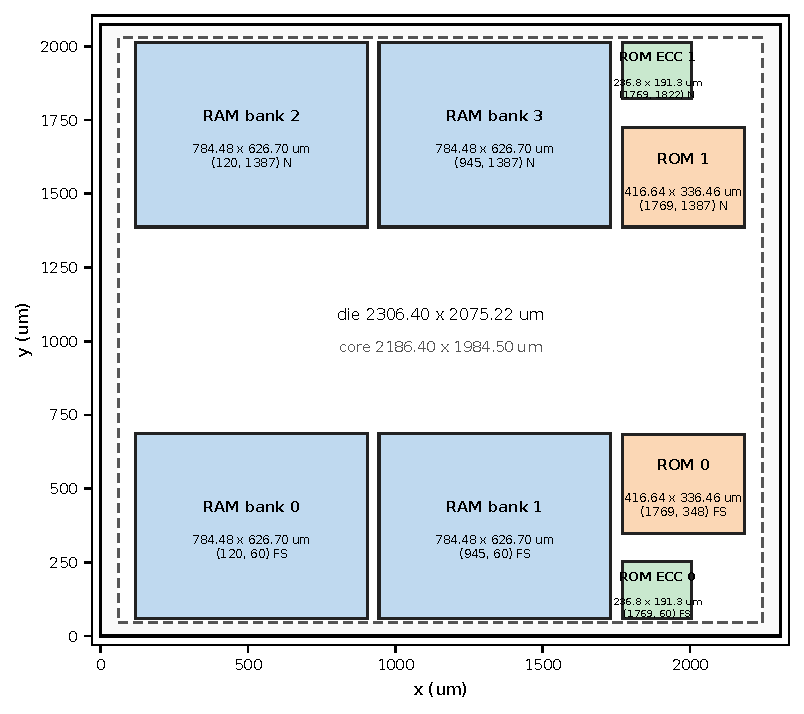
\includegraphics[width=0.70\linewidth]{figures/floorplan_macros.pdf}
\caption{The eight vendor macros with sizes, origins and orientations
on the \SI{2306.40}{}$\times$\SI{2075.22}{\um} die; no
standard cells drawn. The lower row is mirrored so that both rows' pin
edges face the channel between them.}
\label{fig:floorplan}
\end{figure}

\subsection{The floorplan and its five regions}

The die is \SI{2306.40}{}$\times$\SI{2075.22}{\um} =
\SI{4786290}{\um\squared} = \SI{4.79}{\milli\meter\squared},
around a site-aligned core box of \SI{4338910}{\um\squared}.
The eight macros are FIXED; nothing else was told where to go. Two
mirrored macro rows and the ROM column between them and the die edge
partition the placeable area into exactly five regions: the
\textbf{central channel}, \SI{700.08}{\um} tall and the full
core width; the \textbf{lower} and \textbf{upper macro rows}, the
slivers left beside and between the RAM macros; and the \textbf{lower}
and \textbf{upper halves of the ROM column}, the pockets the ROM
macros---shorter than the RAM---leave at the right of each band. Every
non-fill placed instance falls in one of the five, and they sum to
\num{60694}, the whole non-fill population.

\begin{figure}[p]
\centering
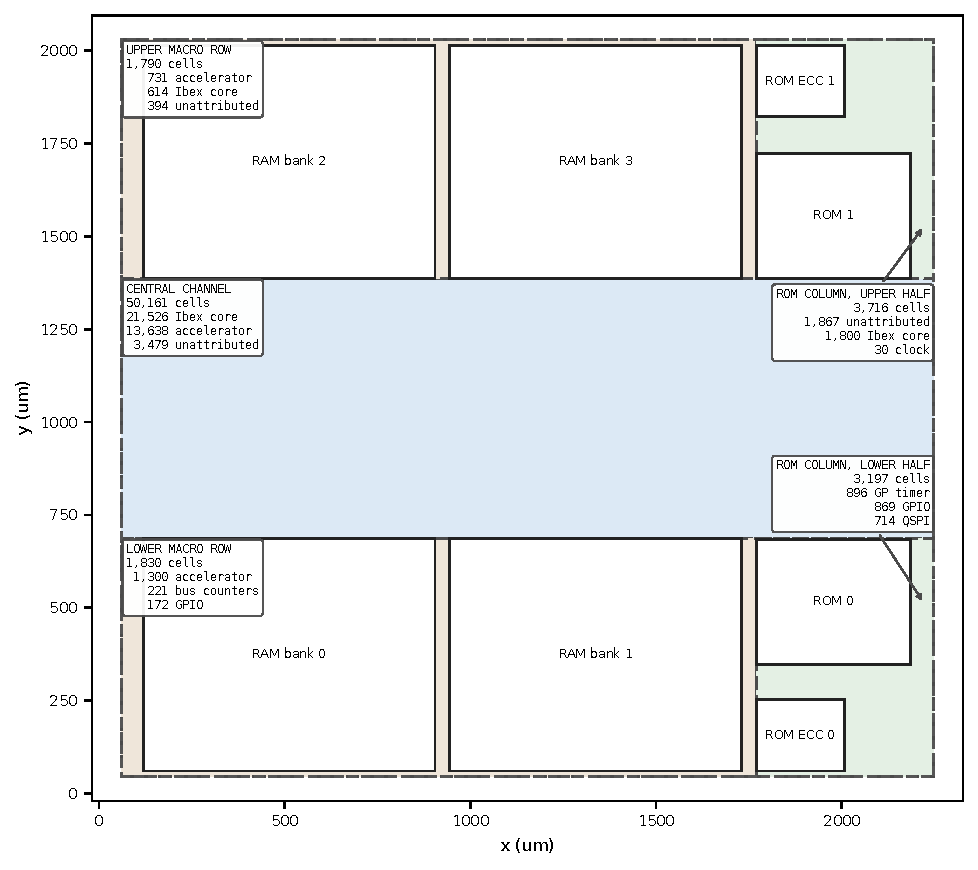
\includegraphics[width=\linewidth]{figures/layout_regions.pdf}
\caption{\textbf{The die by region.} The five regions the floorplan
creates, each annotated with its non-fill cell count and its three
largest occupants, over the placed cells and the eight fixed macros.
Occupancy is counted from the sign-off placement, not assigned by
intent: apart from the macros, nothing here was constrained. The boxes
rank the unattributed and clock-tree classes among the occupants where
they fall, which is why three of the five name the unattributed one and
one of those three also names the clock; Table~\ref{tab:regions} separates the
unattributed share out.}
\label{fig:regions}
\end{figure}

\subsection{The attribution, and the error bar on every block figure}

\textbf{This must be stated before the map is read.} ``Where is the
processor'' is a question about a die carrying \num{168592} instances,
and after this flow's synthesis almost none of them says which block it
came from. Only \num{1140} of those names contain a dot at
all---\num{632} the RAM's and \num{266} the ROM's, tie cells but for
the eight macros themselves, most of the rest clock buffers---and by
the attribution script's own prefix test
\textbf{exactly one instance in the die carries a top-level block
name}: \file{u\_ibex.core\_clock\_gate\_i.u\_icg}, an integrated clock
gate. Everything else is a Yosys name with no block in it, so a picture
colouring only the named instances would colour one cell.

The attribution is therefore by \emph{connectivity}. Yosys renames
cells but keeps the hierarchical name of any net it did not create, so
\num{643} nets still vote for a top-level block; each anonymous cell
takes the block most of its pins' nets vote for; unattributed cells
then take the majority block of their neighbours, twice, which is where
it converges. Clock buffers, tie, tap, fill and decap cells are
recognised by name or master and form their own classes, belonging to
no block.

\textbf{The residual is reported, not hidden.} \num{5916} of the
\num{60694} non-fill instances---\SI{9.747}{\percent}---end
unattributed and are drawn grey. That is the error bar on every
block-level statement here and on every block figure this project has
published, Figure~\ref{fig:panels} included. It is also not uniform,
which nothing has stated before: Table~\ref{tab:regions} gives it per
region, from \SI{0.93}{\percent} in the lower macro row to
\SI{50.24}{\percent} in the upper half of the ROM column. A block count
from that last region is worth little; one from the channel, at
\SI{6.94}{\percent}, is worth a good deal more.

\begin{figure}[p]
\centering
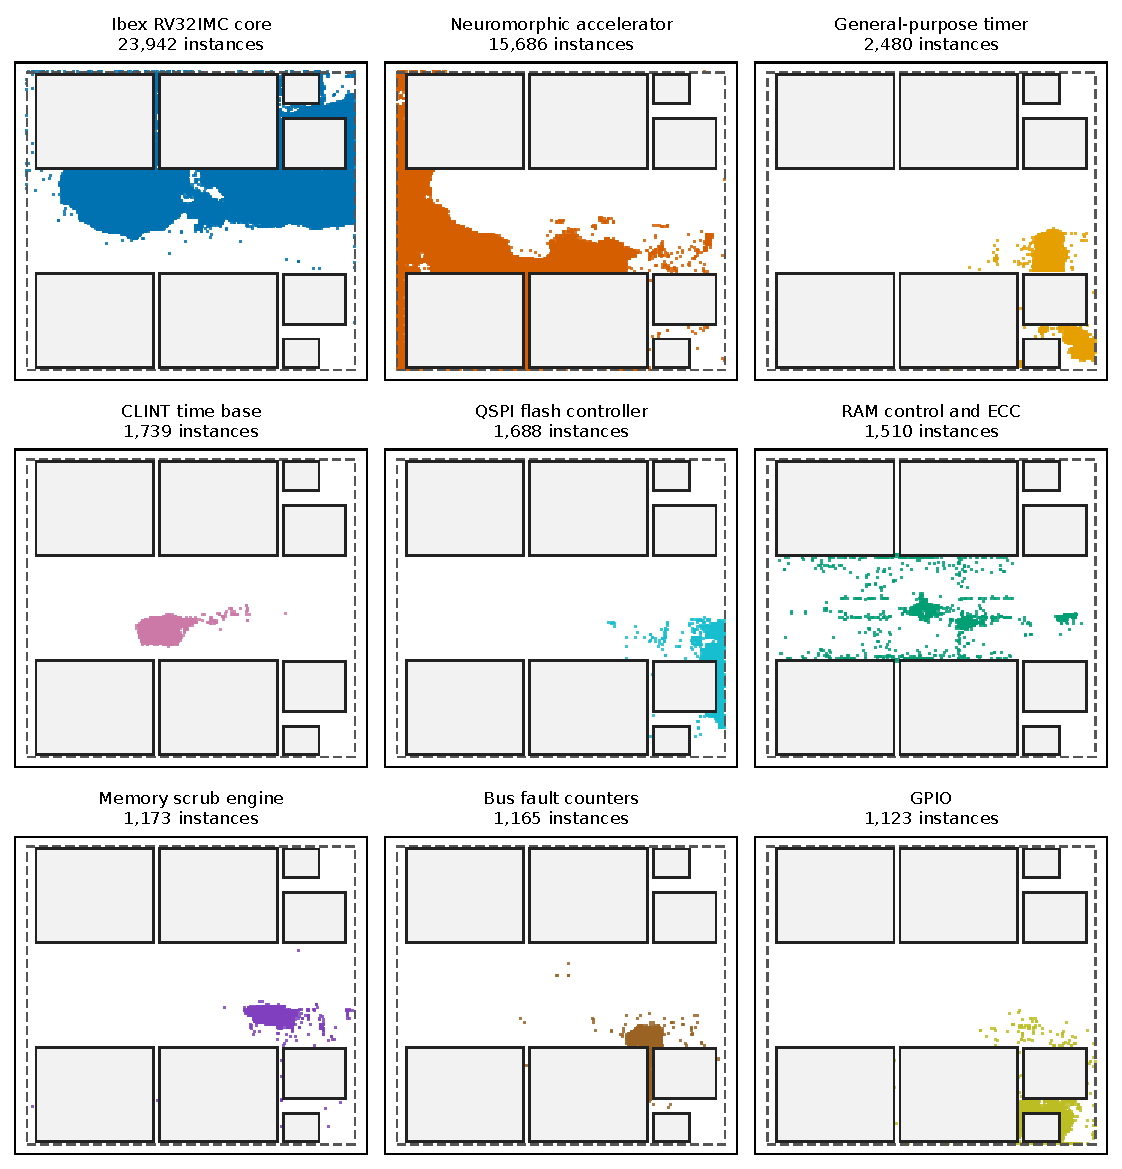
\includegraphics[width=\linewidth]{figures/layout_panels.pdf}
\caption{One panel per block, for the nine largest blocks by attributed
cell count---fourteen clear the script's \num{300}-cell floor and it
keeps the nine biggest---over a grey ground of every other non-fill
instance. These carry the residual of \S\ref{sec:phys}:
\SI{9.747}{\percent} of the non-fill instances are in neither the
coloured set nor any other block's.}
\label{fig:panels}
\end{figure}

\begin{table}[t]
\centering
\small
\begin{tabular}{L{3.4cm}rL{5.5cm}r}
\toprule
region & cells & three largest attributed occupants & unattributed \\
\midrule
central channel & \num{50161} &
  Ibex core \num{21526}; accelerator \num{13638}; CLINT \num{1739} &
  \num{3479} (\SI{6.94}{\percent}) \\
lower macro row & \num{1830} &
  accelerator \num{1300}; bus fault counters \num{221}; GPIO \num{172} &
  \num{17} (\SI{0.93}{\percent}) \\
upper macro row & \num{1790} &
  accelerator \num{731}; Ibex core \num{614}; RAM control \num{4} &
  \num{394} (\SI{22.01}{\percent}) \\
ROM column, lower half & \num{3197} &
  GP timer \num{896}; GPIO \num{869}; QSPI \num{714} &
  \num{159} (\SI{4.97}{\percent}) \\
ROM column, upper half & \num{3716} &
  Ibex core \num{1800}; ROM control \num{18}; accelerator \num{1} &
  \num{1867} (\SI{50.24}{\percent}) \\
\midrule
total & \num{60694} & & \num{5916} (\SI{9.747}{\percent}) \\
\bottomrule
\end{tabular}
\caption{What each region holds, counted from \file{s83romecc5}'s final
DEF and netlist. ``Cells'' is non-fill placed instances: fill, decap,
tie, tap and antenna cells are excluded. The clock tree is not: its
\num{1075} cells belong to no block, so they are inside the ``cells''
column and outside the occupant columns. The unattributed share
is this attribution's own error bar, and it is not uniform. This
project also runs a \emph{different} five-zone census over the same
DEF, which counts \num{64349} standard cells because it excludes only
fill; the two partitions answer different questions and their rows must
not be compared.}
\label{tab:regions}
\end{table}

\subsection{What is in each region, and why}

\paragraph{The channel holds the core and the accelerator, because it
is the only contiguous area.} \num{50161} of \num{60694} non-fill
instances---\SI{82.6}{\percent}---are in the channel, and the two
largest blocks dominate it: \num{21526} of the core's \num{23942}
attributed cells and \num{13638} of the accelerator's \num{15686}. The
placer was not told to do that; the channel is simply the one region
tall and wide enough to take a block of tens of thousands of cells
without splitting it. The overflow goes into the macro rows, where the
accelerator is the largest occupant of both: \num{1300} cells in the
lower row and \num{731} in the upper.

\paragraph{The CLINT's closure is entirely in the channel, which
settles an open question.} A separate census of its \num{1802}-cell
register-to-register closure puts \num{1802} of \num{1802} in the
channel, none in either pocket and none in the strip beside the ROMs.
A prior document had ended with the instruction that keeping that set
on one side of the ROM ``is a floorplan requirement and not a placement
one''. \textbf{It is already met, by the placer, with nothing asked of
it}---and five earlier runs that forced the cluster into a box or moved
a fence were answering a question the eight-macro floorplan had already
answered by accident.

\paragraph{The ROM column's lower pocket is peripheral ground, because
that is where the peripherals' pins are.} Its three largest attributed occupants
are the general-purpose timer (\num{896}), the GPIO port (\num{869})
and the QSPI controller (\num{714}), with the boot controller fourth at
\num{463}. GPIO and the boot controller have their plurality
here---\num{869} of \num{1123} and \num{463} of \num{891}---while the
timer keeps \num{1562} of \num{2480} in the channel and QSPI \num{972}
of \num{1688}: the pocket pulls the peripherals out, it does not hold
them. That is not where a block
diagram would put any of them and it is exactly where the I/O placement
puts their pins. Of
the \num{94} top-level pins in the DEF's \texttt{PINS} section,
\textbf{\num{48} lie below the core box and \num{39} to its
right}---\num{87} of the \num{92} signal pins on the bottom and right
edges---with four on the left, one at the top and the two power pins
inside the core. GPIO alone accounts for \num{42} bottom-edge pins and
seven right-edge ones; QSPI has sixteen, all on the right.
\textbf{There is no pad ring}: these are DEF pin shapes
\SI{0.2}{\um} in from the die boundary, placed by the flow's
I/O placement step, and the design has no pads, no package and no I/O
cells.

And the upper half of the ROM column is where the attribution runs out:
\num{1867} of its \num{3716} cells are unattributed and \num{1800}
attributed to Ibex, which is as much as this method can say.


\subsection{Sign-off}

\begin{table}[t]
\centering
\small
\begin{tabular}{lrrr}
\toprule
corner & setup worst & setup violations & hold worst \\
\midrule
\texttt{nom\_slow\_1p08V\_125C} & \SI{-7.5758}{\nano\second} &
  \num{3529} & \SI{+0.4261}{\nano\second} \\
\texttt{nom\_typ\_1p20V\_25C} & \SI{+2.6396}{\nano\second} &
  \num{0} & \SI{+0.1769}{\nano\second} \\
\texttt{nom\_fast\_1p32V\_m40C} & \SI{+8.3630}{\nano\second} &
  \num{0} & \SI{+0.0296}{\nano\second} \\
\bottomrule
\end{tabular}
\caption{Post-layout static timing on \file{s83romecc5} at the three
corners, on extracted parasitics, with a \SI{5}{\percent} derate
applied as a float and \SI{0.25}{\nano\second} of clock uncertainty,
against a \SI{20}{\nano\second} SDC period. Setup total negative slack
at the slow corner is \SI{-14735.65}{\nano\second}; \textbf{hold has
zero violations at all three corners}. The design also fails max slew
(\num{533}/\num{77}/\num{20} violations at slow, typical and fast), max
capacitance (\num{95}/\num{96}/\num{98}) and max fanout (\num{589} at
every corner, in a flow with no max-fanout checker step at all). Three
of those are visible only because the violation-corner keys were bound
to every corner before the run rather than audited after it; under the
shipped defaults the flow would have printed warnings and exited
zero.}
\label{tab:timing}
\end{table}

\begin{table}[t]
\centering
\small
\begin{tabular}{L{4.3cm}L{9.9cm}}
\toprule
check & result on \file{s83romecc5} \\
\midrule
detailed-route DRC & \num{0}, at the router's iteration \num{16} \\
disconnected pins & \num{0} \\
power-grid violations & \num{0} on both rails \\
antenna, post-route & \num{2} violating nets, \num{2} violating pins;
  \num{1258} diodes inserted \\
routed wirelength & \SI{5746921}{\um}; \num{62767} signal nets
  and two special; \num{486886} vias, all single-cut; longest net
  \SI{4292.89}{\um} \\
Netgen LVS & circuits match uniquely, \num{263} symmetries, all seven
  difference counters \num{0}, with the vendor macros black-boxed on
  both sides---so it signs off the connectivity \emph{into} all eight
  macros' pins and says nothing about their internals \\
KLayout DRC & \num{11048} markers, \num{6584} distinct shapes, and
  \textbf{every one inside the vendor macro hierarchy}; \num{0}
  outside. The deck declares \num{173} rule categories in \num{47}
  groups; three fired \\
Magic DRC, abstracted & \num{170} error boxes, \num{20} inside a macro
  footprint and \num{150} outside---and every one of the \num{150}
  within \SI{0.500}{\um} of a macro edge, none in open routing
  area \\
KLayout XOR & \textbf{not run on this layout}; run on the
  antenna-repaired variant \file{s83ant}, where the difference count is
  \num{0} \\
total power, typical corner & \SI{56.41}{\milli\watt}, \emph{with no
  switching activity annotated} \\
\bottomrule
\end{tabular}
\caption{Sign-off on the eight-macro layout. Route, pin, grid, antenna,
wirelength and power are \file{s83romecc5}'s own metrics; the four deck
rows are decks run on that layout in trees of their own, its
configuration gating all four off---\file{s83lvsbb2}, \file{s83kdrc},
\file{s83mdrc} and, for the XOR, \file{s83antxor}. The two geometric
deck rows need the qualifier the companion
papers carry~\cite{companion_decks}: the vendor SRAM macro does not pass this
PDK's own decks, which is a property of the kit rather than of this
design, so the honest form of a deck result here is two
numbers---inside the macro and outside it---and not one.}
\label{tab:signoff}
\end{table}

Three things travel with Tables~\ref{tab:timing} and~\ref{tab:signoff}.

\textbf{The layout does not meet its setup constraint}, reported with
the same weight as what passes: \SI{-7.5758}{\nano\second} at the slow
corner on \num{3529} violating endpoints against a
\SI{20}{\nano\second} period. The aggregate metric
\texttt{design\_\_violations} nonetheless reads \num{0} in this run's
own metrics file. \textbf{The aggregate metric does not aggregate}, and
a reader who trusted it would conclude the layout was clean.

\textbf{It meets hold at all three corners, and that is not free.}
Raising the antenna repair's iterations and margin clears both antenna
violations---\file{s83ant} reports \num{0} nets and \num{0} pins---for
\num{60} additional diodes, and \emph{loses hold}:
\SI{-0.4351}{\nano\second} on \num{55} endpoints, \num{38} fast,
\num{16} typical, one slow. That is a bad trade, a hold violation being
a functional failure where the two antenna violations it removes are
ratio overshoots, and it cannot be tuned away: repeating the repair at
gentler settings converges on exactly the same layout.

\textbf{The power figure is an estimate wearing a measurement's
clothes.} The flow calls \texttt{report\_power} with nothing having
read a VCD or a SAIF, so \SI{56.41}{\milli\watt} rests on the timer's
default propagated activity and not on any program this project has
run. Activity-annotated measurements on layouts containing the
accelerator give \SI{22.142}{\milli\watt} computing and
\SI{8.287}{}/\SI{8.315}{\milli\watt} idle with the core gated in WFI,
and those are the figures to quote.

\section{What the measurements settle}
\label{sec:settle}

\subsection{No frequency, and now a reason as well as a rule}

This project publishes no clock frequency for this design, and the rule
is its own: a figure published externally must be traceable to
measurement or clearly labelled as a design target, and the only figure
available is a measured \emph{non-closure} from a layout that fails
setup, slew and capacitance. Two further grounds stand: the mission
requirement is a frame rate, and the shuttle tile would carry a
different figure, so publishing two numbers would tell a reader the
project cannot say what its clock is. The \SI{20}{\nano\second} SDC
period is kept as a flow constraint so that four rounds of slack
measurements stay comparable. What \S\ref{sec:settle-fp} adds is the
measured reason.

\subsection{The timing is not a floorplan question}
\label{sec:settle-fp}

Every violating path in the sign-off report was decomposed at its
launch flip-flop's \texttt{Q}, each incremental delay after it
attributed to a cell arc or to a net, with the clock network counted
into neither so the percentages compare across layouts with different
clock trees. Over the \num{1000} violating paths: \textbf{wire is
\SI{1.9}{\percent} of a violating path at the median and
\SI{3.0}{\percent} at the most wire-bound path}, over a median of
\textbf{\num{78} gate stages}, \num{57} to \num{91}. The worst path is
\num{77} stages, \SI{26.2904}{\nano\second} of cell delay and
\SI{0.7827}{\nano\second} of net delay---so if every wire on it were
made ideal it would still take \SI{26.29}{\nano\second} against a
\SI{20}{\nano\second} constraint. A floorplan moves wire; there is no
version of this floorplan that moves \num{78} gate stages. Nor is the
profile an artefact of this one: an earlier layout on a different macro
set, \file{s71boot}, gives \SI{1.9}{\percent} at the median and
\SI{2.8}{\percent} at the maximum over its \num{985} violating
paths. That is the second half of the CLINT result above---the
condition five placement experiments were run to enforce is already
met, and the quantity they could have moved is under \SI{5}{\percent}
of every violating path in any of the three floorplans measured.

\textbf{A correction belongs here.} These figures were first published
on 2026-09-16 as \SI{3.6}{\percent} at the median and
\SI{4.7}{\percent} at the maximum over a median of \num{88} stages,
from a tool that was cutting each path at the end of the report block
instead of at \texttt{data arrival time} and so counting the
\emph{capture} clock's tree into the data path. It was corrected the
same day, and the old figures are an instrument defect rather than a
superseded measurement---nothing about the design changed between them.
Three places in the corpus still carry a pre-correction figure: the
summary section of the document that made the correction and the
opening of the document that cites it carry the \num{88}, and the
document index carries the \SI{3.6}{\percent} beside a corrected
\SI{3.0}{\percent}. All three are named here.

The register file's data bits hold \num{1007} of the \num{3529}
violating endpoints, its SECDED check bits \num{217} and the rest of
Ibex \num{864}---\num{2088} together, \SI{59}{\percent} of the count
and \SI{58}{\percent} of the total negative slack---against \num{54}
for the fabric. \textbf{And the
single worst endpoint is a SECDED check bit of the register file}: read
address, through the core's datapath, into the write encoder, into the
check-bit storage. It is the hardening's own write path, priced in
\S\ref{sec:harden} in area and in fault coverage but never in depth. No
placement removes an XOR tree.

\subsection{The registered request phase buys the depth and does not
route}

The one structural change inside this project's own RTL that the path
decomposition points at is a registered request phase in the fabric:
make the grant and the transfer two events instead of one, so the
slave's decode and read multiplexer start at a flip-flop. It was built
behind a parameter, the default proved unchanged by an equivalence
miter, and the fabric's whole property set proved again at both
settings---the six tasks in Table~\ref{tab:formal}'s \file{soc\_bus}
row.

\textbf{It buys what it was built to buy.} Maximum combinational depth
goes from \num{81} levels to \num{69} and the median from
\textbf{\num{39} to \num{20}}; the deepest endpoint class, the CLINT's
response registers, goes from \num{81} to \num{16}. \textbf{It costs
\SI{24.89}{\percent} of the cycle count}: the same workload runs in
\num{520398} cycles against \num{416673}, passing at both. The register
is a skid buffer, so throughput is unchanged; what grows is latency, by
one cycle, on every transaction.

\textbf{And its layout does not route.} The same netlist through the
same flow with the same configuration and initial state, run
\file{s89rr1}, stops at global routing with congestion: \num{387} overflowing tiles against \num{0}
for the sign-off layout, \num{353} of them on one metal layer, with
total wirelength up \SI{586339}{\um} (\SI{+8.2}{\percent}) for
\num{159} additional nets. Before the change, the fabric's address,
byte-enable and write-data outputs are combinational selections between
two masters, driven from wherever the placer put the masters' own
logic; after it, all three come out of \emph{one} register that must
reach all seven targets---the six slave ports and the internal error
slave---which, as \S\ref{sec:phys} measured, the I/O placement and the
macro column spread to opposite corners of the die.
\textbf{A single point driving a \num{69}-bit bus to seven destinations
is a broadcast, and a broadcast goes on the long layer.} The change
adds wire not because it adds cells but because it moves the fan-out's
origin from two well-placed sources to one.

So the trade on offer is not a quarter of the cycle count against an
unmeasured slack improvement, but a quarter of the cycle count against
a design that stops at global routing, and \textbf{the default stays
off}. The depth result stands, being a netlist measurement independent
of placement; what the layout adds is that \emph{this} way of
delivering it---one register at one point---is what the router cannot
take. A version registering the request at each slave would buy the
same depth without the broadcast; it is not built, and its first
constraint is known before it is.

\subsection{And what none of this is}

Not a flight part and not radiation-hardened. No silicon, no beam, and
the open kit publishes no total-ionising-dose or single-event data, so
every reliability figure in this project is a seeded fault-injection
measurement on a model---including the campaign that once produced
bit-identical output on a defective design and its repair, a companion
paper's subject~\cite{companion_tmr}. The spacecraft interfaces, the
accelerator mesh and any design-for-test are absent, and the vendor
SRAM macro cannot be signed off on this PDK version at all, which is
why Table~\ref{tab:signoff}'s deck rows are two numbers and not one.
The companion paper~\cite{companion_design} carries the full list.

\section{Availability}
\label{sec:avail}

The public repository is \url{https://github.com/Melihakbulut221/nssoc}.

It is a generated mirror of the development tree, carrying the tree and
not the history: the RTL, the testbenches, the formal jobs and their
property files, the flow configurations, the register-map and
memory-map single sources, the golden models and their suite, the
shuttle submission, the numbered document corpus, and the LaTeX sources
of the thesis~\cite{thesis_nssoc} and of every preprint tracked there,
this one included at the mirror's next generation, with the thesis also
shipping as a built PDF. Run trees are not in
it, which is why every physical figure here is quoted with the run tag
it came from.

\textbf{Three things are held back and none is technical}: the
product-line positioning section of one document, the funding and
shuttle commercials of a second, and the drafted text of an unsubmitted
funding application. Each is replaced by a stub keeping the filename and
saying what was held and why, so the documents citing them still
resolve and a reader sees a withholding rather than a silent gap.
\textbf{No negative result, no withdrawn claim, no measurement and no
failing check is held.} That is the condition under which the rest of
the corpus means anything, and it is why this paper can report a layout
that does not close, a remedy that does not route, four formal tasks
killed by hand and eight instructions with no formal result.

\section{Conclusion}
\label{sec:conc}

\textbf{Where it landed.} The channel holds the core and the
accelerator because it is the only contiguous area; the ROM column's lower
pocket is peripheral ground because that is where \num{87} of \num{92}
signal pins are; the CLINT's closure is entirely in the
channel, which retires five placement experiments. Each is a
connectivity attribution carrying a \SI{9.747}{\percent} unattributed
remainder, reported per region because it is not uniform: a die map of
a flat netlist is an inference, and this one states its own error bar.

\textbf{What was proved.} \num{86} tasks across \num{20} property sets,
counted from the job files: conformance and masking as theorems,
invariants over all reachable states for what a test can only sample,
one event-engine invariant closed in \SI{5}{\second} that two documents
had declined to close, one register-file job that does not close
because parity is where the solver stops, and eight M-extension
instructions with no formal result. And two negative results worth more
than either: the timing is not a floorplan question, and the one
structural remedy this project's own RTL can reach halves the median
logic depth, costs a quarter of the cycle count, and does not route.
Both are published, because a record carrying only what worked is not a
record.

\bibliographystyle{plain}
\bibliography{refs}

\end{document}
